\begin{design}
\section{Design Overview}
Based on the project specification, there are a number of important functions the library needs to provide. These functions can be summarized in a flowchart (figure 3). The following subsections will move down the flowchart, discussing the planned design and architecture of each component.
\begin{figure}[h]
    \centering
    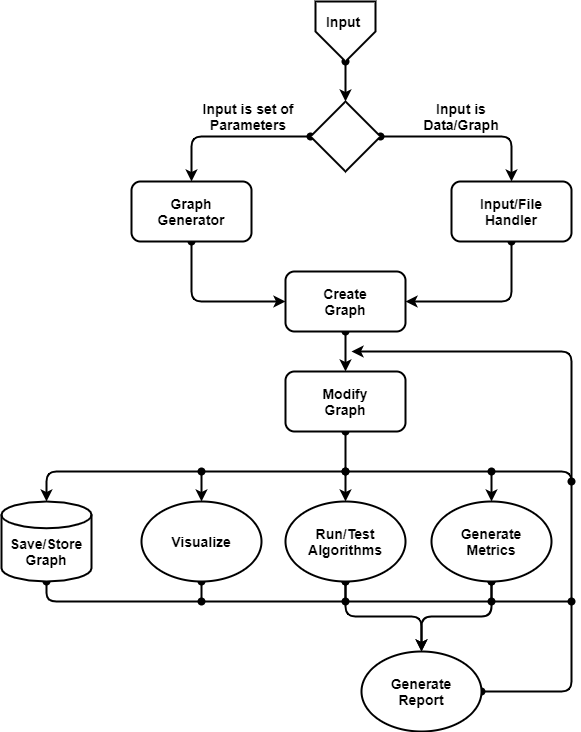
\includegraphics[scale=0.58]{images/flowchart.png}
    \caption{Functionality flowchart.}
\end{figure}
\subsection{Input}
The flowchart input can be of multiple types; raw temporal data that has been collected from a system, a previously created graph that was stored in a file, or a set of parameters for a graph generator. Given that there are expected to be many types of input formats, a modular approach to input handling is required. Each type of input should handled with a new subclass and produce the same set of outputs for graph creation. The parent input class should hold any properties and methods that are common across all inputs.
\subsection{File Handler}
Each file format will be handled by creating an input handler subclass from the input class. For example, if the input is a .csv file with a list of time-edges (figure 5), then this should be handled using the CSVInput class (figure 4).
\begin{figure}[h]
  \centering
  \begin{minipage}[b]{0.4\textwidth}
    \centering
    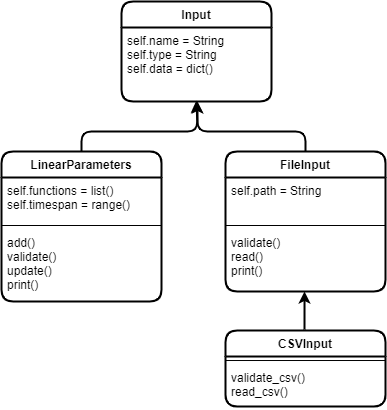
\includegraphics[scale=0.6]{images/UML_input.png}
    \caption{Example input handlers.}
  \end{minipage}
  \hfill
  \begin{minipage}[b]{0.4\textwidth}
    \centering
    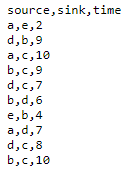
\includegraphics[scale=0.8]{images/csv.PNG}
    \caption{Sample csv file; list of time-edges.}
  \end{minipage}
\end{figure}
A common output format across the input handler classes would be very useful. This would allow for the construction of the graph to remain the same for an ambiguous set of inputs, as each input is handled within its own class. Any input validation unique to the input should also be added to this class, prior to passing the output to the graph constructor.
\subsection{Generators}
As mentioned in the specification, there are multiple methodologies available for generating temporal networks. Two examples are random generation of time-edges, and the generation of time-edges from a set of linear functions. Each generator would be defined as a class and produce the same output format  in order to remain compatible with the graph constructor. This allows an ambiguous set of generators to be created/defined without having to redesign the graph constructor for each.
\subsection{Graph Construction}
The construction of a temporal graph can be achieved in multiple ways. One idea is to simply store all the time-edges in a data structure, such as a dictionary, as a property of a temporal graph object. Another is to create a static graph for every instance of (discrete) time, or over a set of time intervals. These static snapshots could be represented in a class, and added into a data structure which would be stored as a property of the temporal graph object.\\
The chosen architecture looks at the temporal graph at a more granular level; modelling the components of the graph. Static graphs are built from nodes and edges, while temporal graphs are built from nodes and time-edges/links. The idea is that one could create a base class definition for nodes and edges, and then extend that definition to the temporal domain. Further extensions could also be realized for other graph constructions, custom specifications and use-cases.\\
This modular building block approach offers a flexible and powerful way of expressing a graph.
\begin{figure}[t]
    \centering
    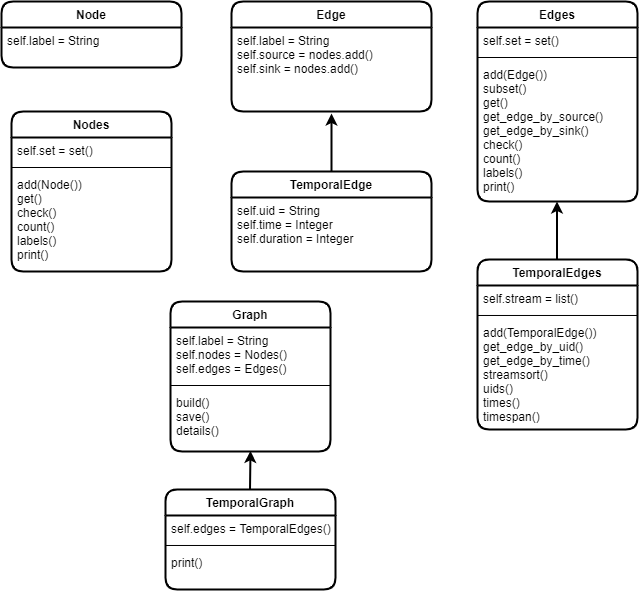
\includegraphics[scale=0.7]{images/UML_graph_components.png}
    \caption{Graph components and graph UML diagram.}
\end{figure}
Figure 6 shows some basic class definitions for the components of the Graph and TemporalGraph classes (digraph and discrete digraph respectively). A Graph has the properties nodes and edges, which are classes that define collections of the Node and Edge components. Nodes describes a set of Node objects, each of which has a label property. Similarly, Edges describes a list of Edge objects, each of which has a label, source, and sink property (here we are dealing with directed edges). The source and sink of an Edge object are Node objects themselves, stored in a Nodes collection. The idea here is that, when adding an Edge to a graph, the graph's Nodes collection is passed as a parameter, in order to maintain and update the graph's nodes. This process occurs in the constructor method of the Edge class.\\
For the TemporalGraph definition, the edges property is simply replaced with the TemporalEdges class, which is a subclass of the Edges class. TemporalEdges is a stream (list, ordered by time) of TemporalEdge objects. TemporalEdge is a subclass of Edge, with some new properties, such as uid (label name + time), time (discrete) and duration (discrete). By construction, the TemporalGraph class is already fundamentally different than that of the Graph class, which is expected and was mentioned in the introduction. When building the graph, the nodes and edges are connected through the edge properties source and sink, while adding the edges themselves. Any unconnected nodes can then be added afterwards by directly calling the Nodes add() method. All the information required to build the graph will be passed from the input handler object data property (figure 4).
\subsection{Graph Functions}
The created graph can have a number of functions associated with the overall graph, and the components themselves. Typical graph functions include printing the graph details, and generating a visualization. The edges can be retrieved through methods like graph.edges.get\_edge\_by\_source('b'), graph.edges.get\_edge\_by\_sink('a'), graph.edges.get\_edge\_by\_time(3). Nodes can be retrieved through graph.nodes.get('x'). Each of these methods returns a new Edges/Nodes collection, which is a subset of the graph itself. All of the methods are callable on the subset. Figure 7 demonstrates this functionality.
\begin{figure}[h]
    \centering
    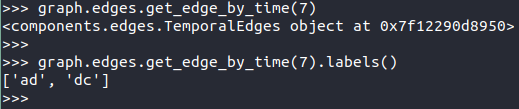
\includegraphics[scale=0.7]{images/graph_get_edge_labels.PNG}
    \caption{Graph functions example.}
\end{figure}

\subsection{Graph Modification}
New nodes and edges can be added to the graph through the respective add() functions of the collection classes. Similarly, nodes and edges should be removable from the graph, taking care to handle any unconnected edges. Furthermore, the properties of edges and nodes should be editable, provided the edit is valid and does not violate graph integrity or any added constraints. 
\subsection{Saving a Graph}
The Graph class includes a save() method, which will run through the graph components and save all structural information (basic save) into a file, including any new metrics generated during the session (full save). The file can also include a complete summary of the graph. By saving into a specified format, the graph should be reproducible from the file.
\subsection{Visualization}
It is important for the user to be able to visualize the graph, or subsections of the graph. Visualization can provide a means of quick verification by the user to see if the graph has been created or modified correctly. It can also aid in the verification of any results produced in testing. A simple command line means of visualization is shown in figure 8. Ultimately, the library would allow for circle \cite{circle_plot} and slice plots (figure 2) of the graph, by using the matplotlib package. The circle plots could be generated for each time step and the resulting images combined into a .gif format or displayed in sequential time, to produce a dynamic plot of the network. Effective visualization may be challenging as larger networks become increasingly more complex. Some examples of circle and slice plots can be found at the teneto github \cite{teneto}, using a combination of circles and Bézier curves.
\begin{figure}[t]
  \centering
  \begin{minipage}[b]{0.4\textwidth}
    \centering
    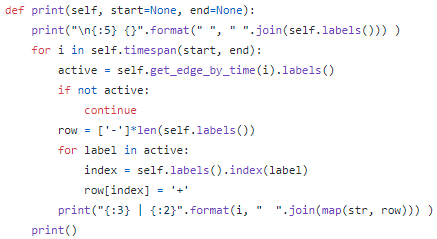
\includegraphics[scale=0.7]{images/graph_print_code.PNG}
    \caption{Basic visualization; edges print method.}
  \end{minipage}
  \hfill
  \begin{minipage}[b]{0.4\textwidth}
    \centering
    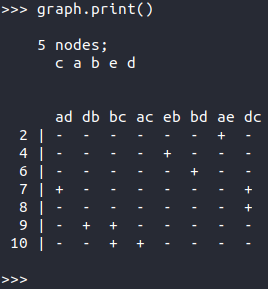
\includegraphics[scale=0.58]{images/graph_print.PNG}
    \caption{Text-based link activity matrix for a discrete temporal network.}
  \end{minipage}
\end{figure}
\subsection{Algorithms \& Metrics}
The algorithm below calculates the foremost time and foremost path from the specified root node to all other nodes in the graph, between a specified time interval. The resulting graph created is the foremost tree of the selected root node. As the algorithm moves through the time-ordered stream of edges within the graph, the edge's foremost time is compared with the current stored time for the destination node (initialized at $\infty$), assuming that the sum of the edge start time and duration is within the specified interval. If the edge's foremost time is lower that the current stored one, the foremost time and the departure node are updated in the foremostTree dictionary under the destination node's entry. This process continues until either the edge times are greater than the upper bound of the interval, or until all the edges have been processed.\\
\vspace{0.1cm}
\begin{algorithm}[H]
\SetAlgoLined
\caption{Foremost time/foremost path algorithm (s4.2 \cite{efficient_algorithms}, modified).}
\KwIn{An edge-stream representation of the graph, a time interval $(t_\alpha, t_\omega)$, a root node x.}
\KwOut{A foremost tree for root node x.}
 initialize $foremostTree[v][time]=\infty$ for all $v\ \epsilon\ V$, \\
 \hspace{1.5cm}$foremostTree[x][time]=t_\alpha$, and $foremostTree[x][source]=x$\;
 \ForEach{edge $e=(u, v, t, \lambda)$ in the edge stream}{
  \uIf{$t+\lambda \leq t_\omega$ and $t \geq foremostTree[u][time]$}{
    \uIf{$t+\lambda < foremostTree[v][time]$}{
        $foremostTree[v][time] \longleftarrow t+\lambda$\;
        $foremostTree[v][source] \longleftarrow u$\;
    }
  }
  \uElseIf{$t \geq t_\omega$}{
    break\;
  }
 }
 \Return{foremostTree for root node x}\;
\end{algorithm}
\vspace{0.1cm}
This example represents a typical case of the algorithms that will be added to the library for graph analysis, and was implemented in order to better understand what classes, properties and methods were required in the core library's architecture. Figure 10 shows the initial implementation, and figure 11 shows the resulting output. The inputs to the algorithm were the graph from figure 9, the source node 'a' and the total time span of the graph. The resulting dictionary provides a foremost tree from node 'a' to every other node in the graph (note: the duration of each edge is 1). For example, the earliest you can be at node 'c' from node 'a' is at time 8. This is achieved by moving along the path $(a \to e \to b \to d \to c )$. It can be noted by looking at the graph that there is another path from $(a \to d \to c)$, but this journey only arrives at node 'c' by time 9 and is therefore not the foremost path.
\clearpage
\begin{figure}[t]
  \centering
  \begin{minipage}[b]{0.4\textwidth}
    \centering
    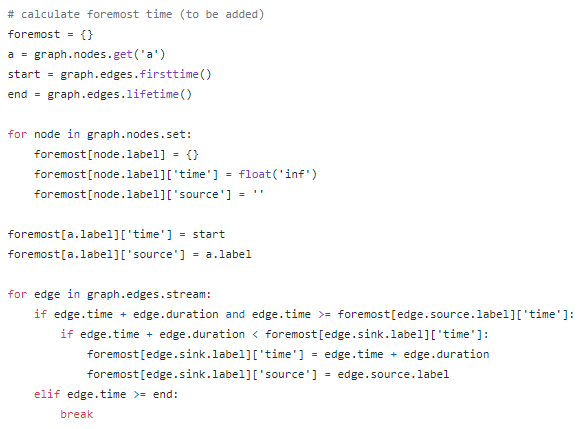
\includegraphics[scale=0.8]{images/foremost_code.PNG}
    \caption{Initial foremost time/foremost path implementation.}
  \end{minipage}
  \hfill
  \begin{minipage}[b]{0.4\textwidth}
    \centering
    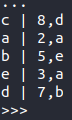
\includegraphics[scale=0.7]{images/foremost_result.PNG}
    \caption{Resulting dictionary.}
  \end{minipage}
\end{figure}
The finalized implementation would be wrapped in an algorithm subclass, with the data structure for the result in the form of a foremost tree object. Other algorithms for calculating network centrality, latency, connectivity and reachability could also be created as algorithm subclasses. Each of these subclasses would produce its respective metrics in a standardized format.
\subsection{Reports}
The results of any measurements and algorithms run/tested on the graph should be printable in an intuitive and clear format. This can be handled through a report class definition.
\subsection{Design Evaluation}
Verification of the code can be achieved by testing all the methods individually and by writing unit tests \cite{unittest}. The unit tests (or tests in general) should be documented within the library with an example, to encourage a standardized test format. Any algorithms implemented can be tested on a suitable test case temporal network and verified visually and through careful experimentation. The test case network should be small enough to allow for easy verification, but complex enough to allow for good test coverage. An idea for a test case would be a transport network timetable.
\clearpage
\subsection{Open-source checklist}
\begin{itemize}
  \item Code:\\
  The code will be written in a consistent convention, such as the PEP8 style guide \cite{pep8}. The code should also be well commented, with a clear naming convention.
  \item Documentation:\\
  The library will be well-documented and include a readme, contributing, and code of conduct.
  \item License:\\
  The library will include a license file with a suitable open-source license.
  \item Library name:\\
  The name of the library will be easy to remember, relevant to the library domain and will not conflict with other libraries or trademarks.
  \item Further information about the guide being followed can be found at 'opensource.guide' \cite{open_source}.
\end{itemize}
\subsection{Notes}
\begin{itemize}
  \item Initial library:\\
  The initial library will be created for discrete time, directed temporal networks.
  \item Continuous time:\\
  The library can be expanded to deal with continuous time networks, time-permitting.
  \item Undirected/directed graphs:\\
  The above examples deal with directed graphs. Undirected graph class definitions can be added to the library.
  \item Modular design:\\
  Overall, it is important to ensure the library is designed in a modular fashion, as there is the potential for multiple contributors to be working on it in the future. This also makes the library easier to maintain.
  \item Efficiency:\\
  Any methods implemented that perform some function on the network will be developed with efficiency in mind. The modelling and analysis of larger networks should not be grossly hindered by the library's performance.
\end{itemize}
\end{design}
\clearpage